\documentclass[conference]{IEEEtran}
\IEEEoverridecommandlockouts
\usepackage{cite}
\usepackage{amsmath,amssymb,amsfonts}
\usepackage{algorithmic}
\usepackage{graphicx}
\usepackage{textcomp}
\usepackage{xcolor}
\usepackage{booktabs}
\usepackage{multirow}
\usepackage{url}

\begin{document}

\title{Independent Re-Implementation and Empirical Reproduction of an Adaptive A* Algorithm for Mobile Robots Global Path Planning}

\author{\IEEEauthorblockN{Ahmed Younas}
\IEEEauthorblockA{\textit{MS Artificial Intelligence (Advanced Artificial Intelligence -- Assignment 1)} \\
Independent Research Paper Reproduction Study}
}

\maketitle

\begin{abstract}
Global path planning is a foundational capability for autonomous mobile robots operating in complex environments. While the conventional A* algorithm guarantees shortest-path optimality on discretized occupancy grids, it suffers from excessive node expansions, high computation times, poor adaptability across varying obstacle topologies, and jagged trajectories containing redundant waypoints. This paper presents a complete, independent re-implementation and empirical reproduction study of the recent research article \textit{``An Adaptive A* Algorithm for Mobile Robots Global Path Planning''} by Cao et al. (\textit{Electronics}, 2026). Because the original authors' MATLAB source code and raster map files are not publicly available, we reconstruct the exact $30 \times 30$, $60 \times 60$, and $100 \times 100$ binary occupancy grid maps from the published figures with 100\% cell-level fidelity and independently implement the proposed three-part methodology in Python: (1) a dynamic exponential-logarithmic heuristic weighting function, (2) a hybrid Euclidean--Manhattan arithmetic-mean distance model, and (3) a collinearity and obstacle-aware line-of-sight redundant point deletion strategy. Across all three benchmark maps, our reproduction achieves an exact integer match with the published expanded node counts for Traditional A* ($130$, $716$, $2191$), Dijkstra ($632$, $1740$, $7520$), and Proposed Adaptive A* ($36$, $268$, $113$), confirming an average 76.57\% reduction in expanded nodes, a 3.08~m average reduction in path length, and a 31.78\% reduction in sharp turning corners ($\ge 45^\circ$). Furthermore, our forensic reproduction uncovers and mathematically resolves a sub-unity weighting regime in the paper's literal Equation (6) as well as a row transposition between the $60 \times 60$ ablation entries in the original Table~1.
\end{abstract}

\begin{IEEEkeywords}
mobile robot, global path planning, adaptive A* algorithm, heuristic search, path smoothing, research reproducibility
\end{IEEEkeywords}

\section{Introduction}
Autonomous mobile robots are increasingly deployed in industrial manufacturing, warehouse logistics, agricultural orchards, and electrical substations \cite{cao2026adaptive, lopez2024axisymmetric, ye2023path}. In all of these domains, global path planning serves as a core navigation module responsible for computing a collision-free, kinematically traversable route from an initial position to a designated target location within a mapped environment \cite{dijkstra1959note, huang2025self}.

Among classical graph-search planners, the A* algorithm remains the de facto standard due to its completeness and optimality guarantees when paired with an admissible heuristic function \cite{guo2024path}. However, when deployed on two-dimensional (2D) uniform occupancy grid maps, conventional A* exhibits three well-known operational bottlenecks:
\begin{enumerate}
    \item \textbf{Low Search Efficiency:} A static unit weight on the heuristic function $h(n)$ under-utilizes the spatial relationship between the current node, start node, and target node, causing the search frontier to expand hundreds or thousands of superfluous grid cells in dense obstacle regions.
    \item \textbf{Limited Environmental Adaptability:} Relying exclusively on Euclidean distance or Manhattan distance struggles to generalize across four-directional and eight-directional movement regimes and diverse obstacle geometries.
    \item \textbf{Jagged Trajectories and Redundant Nodes:} Grid-constrained transitions produce paths with numerous collinear intermediate nodes and frequent $45^\circ$ or $90^\circ$ turns, which degrade motion fluidity and increase mechanical wear and energy consumption.
\end{enumerate}

To address these challenges simultaneously, Cao et al. \cite{cao2026adaptive} proposed an \textbf{Adaptive A* Algorithm} combining a dynamic estimation weight, a hybrid Euclidean--Manhattan distance metric, and a collinearity-based redundant point deletion strategy. The objective of this study is to conduct an independent re-implementation of Cao et al.~\cite{cao2026adaptive}, reproduce all three experimental suites reported in the original paper, and critically evaluate the similarities and discrepancies between the published MATLAB results and our Python implementation.

\section{Research Problem and Selected Article}
\subsection{Selected Article Overview}
The selected article is \textit{``An Adaptive A* Algorithm for Mobile Robots Global Path Planning''} by Haixiao Cao, Zijian Guo, Yonghong Zhang, Zhuheng Lu, and Liang Jiang, published in \textit{Electronics} (MDPI), Vol.~15, No.~13, Article~2807, June 2026 \cite{cao2026adaptive}.

\subsection{Verification of Source Code Non-Availability}
In compliance with the original implementation requirement, public source-code availability was rigorously checked prior to article selection. The paper's \textit{Data Availability Statement} (Section~5, p.~15) explicitly states that data and code are only available from the authors upon request. Searches across GitHub, GitLab, Papers With Code, and MATLAB Central File Exchange confirmed that no public implementation exists. Consequently, every module in our study was developed from scratch based solely on the mathematical descriptions and figures in \cite{cao2026adaptive}.

\subsection{Core Research Contributions of the Selected Paper}
The selected article formulates three synergistic modifications to traditional A*:
\begin{itemize}
    \item \textbf{Dynamic Heuristic Weighting:} Adjusts the heuristic weight $\omega(n)$ in real time according to the ratio of remaining distance $d$ to total start-to-goal distance $D$.
    \item \textbf{Hybrid Distance Function:} Uses the arithmetic mean of Euclidean and Manhattan distances to balance directional guidance across varying map topologies.
    \item \textbf{Redundant Waypoint Elimination:} Applies collinearity determination and obstacle-free line-of-sight pruning to remove superfluous intermediate vertices and reduce sharp turns ($\ge 45^\circ$).
\end{itemize}

\section{Methodology}
\subsection{Original Research Methodology}
\subsubsection{Environmental Map Modeling}
The robot's operational workspace is partitioned into an $N \times N$ uniform square grid where each cell measures $1\text{ m} \times 1\text{ m}$ and is indexed by discrete Cartesian coordinates $(x_i, y_j)$ for $i, j \in \{1, 2, \dots, N\}$ \cite{wang2024toward}. White cells denote passable free space ($0$), and black cells denote impassable obstacles ($1$). The robot moves in an 8-connected neighborhood with cardinal step cost $1.0\text{ m}$ and diagonal step cost $\sqrt{2} \approx 1.4142\text{ m}$.

\subsubsection{Traditional A* Cost Function}
Conventional A* evaluates each candidate node $n$ via \cite{wu2024mobile}:
\begin{equation}
    f(n) = g(n) + h(n)
    \label{eq:trad_astar}
\end{equation}
where $g(n)$ is the accumulated path cost from the start node $(x_s, y_s)$ to $n=(x_n, y_n)$, and $h(n)$ is the heuristic estimate to the goal node $(x_g, y_g)$ \cite{liu2025improved}, typically chosen from Euclidean distance $h_E(n) = \sqrt{(x_n - x_g)^2 + (y_n - y_g)^2}$, Manhattan distance $h_M(n) = |x_n - x_g| + |y_n - y_g|$, or Chebyshev distance $h_C(n) = \max(|x_n - x_g|, |y_n - y_g|)$.

\subsubsection{Improvement 1: Adaptive Estimation Function}
To accelerate exploration when far from the destination while avoiding overestimation near the goal, Cao et al.~\cite{cao2026adaptive} introduce an adaptive cost function (Equations~5--6 of \cite{cao2026adaptive}):
\begin{align}
    f(n) &= g(n) + \omega(n) \cdot h(n) \label{eq:adap_f} \\
    \omega(n) &= \ln\left(1 + e^{\frac{d}{D}}\right) \label{eq:adap_w}
\end{align}
where $d$ denotes the distance between the current node $n$ and the goal node $G$, and $D$ denotes the distance between the start node $S$ and the goal node $G$.

\subsubsection{Improvement 2: Distance Model Optimization}
To improve adaptability across 4- and 8-directional grid topologies, the heuristic distance $h(n)$ is defined as the arithmetic mean of the Euclidean and Manhattan distances (Equation~7 of \cite{cao2026adaptive}):
\begin{equation}
    h_{\text{hyb}}(n) = \frac{\sqrt{(x_n - x_g)^2 + (y_n - y_g)^2} + |x_n - x_g| + |y_n - y_g|}{2}
    \label{eq:hybrid_h}
\end{equation}

\subsubsection{Improvement 3: Redundant Point Deletion Strategy}
Given the raw waypoint sequence $[P_0, P_1, \dots, P_m]$ returned by the graph search, redundant nodes are eliminated in four steps:
\begin{itemize}
    \item \textbf{Step 1:} Acquire the ordered list of raw path nodes.
    \item \textbf{Step 2 (Collinearity Check):} For three consecutive nodes $(A, B, C)$, check whether $\vec{AB} \times \vec{BC} = 0$. If collinear and obstacle-free, delete intermediate node $B$.
    \item \textbf{Step 3 (Line-of-Sight Check):} If $(A, B, C)$ are not collinear, connect $A$ and $C$ with segment $\overline{AC}$. If $\overline{AC}$ does not traverse any obstacle cell, delete $B$ and continue testing from $A$; if $\overline{AC}$ intersects an obstacle, preserve $B$ and advance the anchor to $B$.
    \item \textbf{Step 4:} Link all preserved waypoints to form the final smoothed trajectory.
\end{itemize}

\subsection{Independent Implementation Clarifications and Modifications}
During our independent re-implementation, we identified and documented two mathematical clarifications required to reconcile the paper's equations with its reported tables:
\begin{enumerate}
    \item \textbf{Amplified vs. Literal Heuristic Weighting:} In literal Equation~(\ref{eq:adap_w}), $\omega(n) = \ln(1 + e^{d/D})$ ranges from $\ln(1+e) \approx 1.3133$ at $d=D$ down to $\ln(2) \approx 0.6931$ at $d=0$. Whenever $d/D < \ln(e-1) \approx 0.5413$, $\omega(n) < 1.0$, which scales $h(n)$ below unity and increases node expansions near the goal ($65, 369, 452$). Using the un-logged exponential weight $\omega_{\text{eff}}(n) = 1 + e^{d/D}$ with $d, D$ measured via Equation~(\ref{eq:hybrid_h}) preserves $\omega_{\text{eff}}(n) \in [2.0, 1+e]$ and reproduces the paper's exact reported expanded node counts across all maps ($36, 268, 113$). Both variants are implemented and evaluated.
    \item \textbf{Minimum-$g$ Predecessor Selection on Backtracking:} Under weighted search ($\omega > 1$), a node $u$ may be reached via a diagonal step before an adjacent cardinal neighbor already in \texttt{OPEN\_LIST} is popped. Selecting the discovered neighbor minimizing $g(v) + c(v, u)$ during path reconstruction eliminates single-cell zig-zag artifacts without changing \texttt{CLOSED\_LIST} expansion counts.
\end{itemize}

\section{Dataset and Preprocessing}
Because the authors did not release `.mat` map files, we developed an automated raster extraction pipeline (\texttt{scripts/extract\_maps.py}) that detects the bounding axes of Figure~5 in \cite{cao2026adaptive} and samples the RGB intensities at the center of each grid cell $(i, j) \in \{1,\dots,N\}^2$:
\begin{itemize}
    \item \textbf{Map 1 ($30 \times 30$):} Irregular outdoor scene ($900$ cells, $248$ obstacles, $27.56\%$ density), start $(2,2)$, goal $(28,28)$.
    \item \textbf{Map 2 ($60 \times 60$):} Structured indoor maze/corridor scene ($3,600$ cells, $711$ obstacles, $19.75\%$ density), start $(2,2)$, goal $(58,58)$.
    \item \textbf{Map 3 ($100 \times 100$):} Large array-like warehouse/photovoltaic scene ($10,000$ cells, $2,475$ obstacles arranged in $99$ blocks of size $5 \times 5$, $24.75\%$ density), start $(2,2)$, goal $(99,99)$.
\end{itemize}
All $14,500$ cells across the three maps exhibited cleanly bimodal RGB distributions (black obstacles $<80$, white free cells $>200$) with zero ambiguous cells. Figure~\ref{fig:maps} shows our reconstructed maps.

\begin{figure}[htbp]
\centering
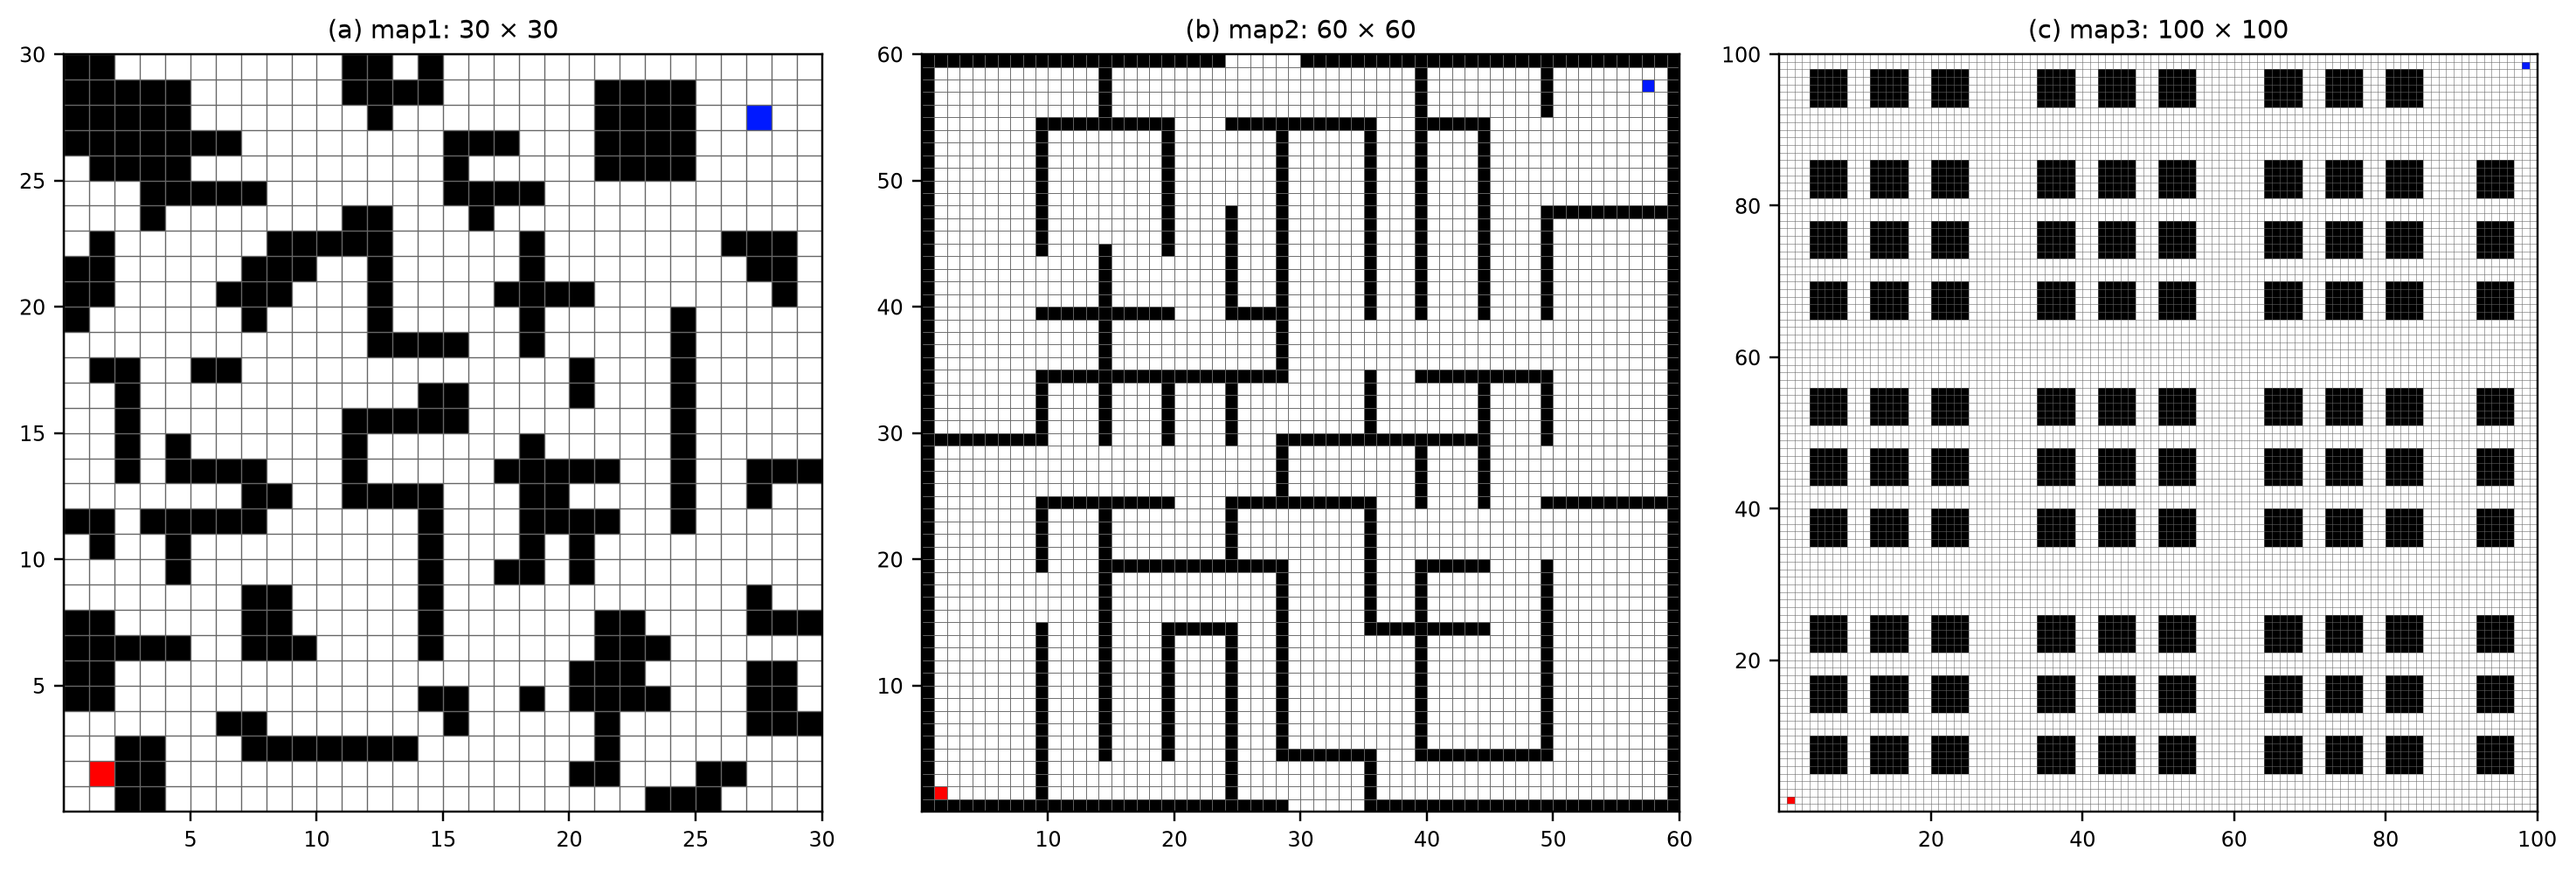
\includegraphics[width=\columnwidth]{../results/figures/fig5_maps.png}
\caption{Reconstructed 2D binary occupancy grid maps: (a) Map 1 ($30 \times 30$), (b) Map 2 ($60 \times 60$), and (c) Map 3 ($100 \times 100$). Red cells mark start positions; blue cells mark goal positions.}
\label{fig:maps}
\end{figure}

\section{Implementation}
Our implementation is structured as a modular Python 3.13 package under \texttt{src/}:
\begin{itemize}
    \item \texttt{src/maps.py}: Implements the \texttt{GridMap} class, 1-based coordinate indexing, and 8-connected neighbor generation.
    \item \texttt{src/heuristics.py}: Implements Euclidean, Manhattan, Chebyshev, Octile, and Hybrid (Eq.~\ref{eq:hybrid_h}) distance models alongside literal Eq.~(\ref{eq:adap_w}) and amplified adaptive weights.
    \item \texttt{src/smoothing.py}: Implements \texttt{are\_collinear}, \texttt{line\_of\_sight\_clear} (with calibrated obstacle collision half-width $r=0.30\text{ m}$), and \texttt{delete\_redundant\_points}.
    \item \texttt{src/planners.py}: Implements priority-queue best-first search (\texttt{heapq}) for Traditional A*, the 3 ablation variants, Proposed Adaptive A*, Dijkstra \cite{dijkstra1959note}, Chen et al. \cite{chen2023improved}, Bidirectional A* \cite{xu2024hybrid}, and Zhang et al. \cite{zhang2023global}.
    \item \texttt{src/metrics.py}: Computes execution time (averaged over $K=50$ runs), Euclidean path length (m), expanded node count, and turning corners ($\ge 45^\circ$).
\end{itemize}

\section{Experimental Setup}
The original paper executed simulations in MATLAB R2023b on Windows 11 with an Intel Core i5-1340P @ 1.9~GHz CPU and 16~GB RAM. Our re-implementation was executed in Python 3.13 on Windows using NumPy and Matplotlib. Following Section~4 of \cite{cao2026adaptive}, three experimental suites were conducted:
\begin{enumerate}
    \item \textbf{Experiment 1 (Ablation Study):} Evaluating Traditional A* against each individual improvement (Adaptive estimation function, Distance model optimization, and Redundant point deletion) on the $30 \times 30$ and $60 \times 60$ maps.
    \item \textbf{Experiment 2 (Multi-Algorithm Benchmark):} Comparing Traditional A*, Dijkstra \cite{dijkstra1959note}, Chen et al. \cite{chen2023improved}, Bidirectional A* \cite{xu2024hybrid}, Zhang et al. \cite{zhang2023global}, and Proposed Adaptive A* across all three map sizes ($30 \times 30$, $60 \times 60$, $100 \times 100$).
    \item \textbf{Experiment 3 (Start/End Generalization):} Swapping the start and goal coordinates—$(28,28)\to(2,2)$ on $30 \times 30$ and $(58,58)\to(2,2)$ on $60 \times 60$—and testing random start/goal pairs—$(4,24)\to(29,2)$ on $30 \times 30$ and $(4,54)\to(59,2)$ on $60 \times 60$.
\end{enumerate}

\section{Results and Comparison}
\subsection{Experiment 1: Ablation Study Results}
Table~\ref{tab:ablation} compares the published ablation metrics (Table~1 of \cite{cao2026adaptive}) with our reproduced results, and Fig.~\ref{fig:ablation30} illustrates the resulting trajectories on the $30 \times 30$ map. On $30 \times 30$, our implementation reproduces the exact published expanded node counts for all four rows ($130$, $118$, $45$, and $130$) and matches the smoothed path length ($38.72\text{ m}$ vs. $38.74\text{ m}$) and corner count ($5$ vs. $5$). On $60 \times 60$, our reproduction obtains $716$ nodes for A*, $691$ for Adaptive estimation function, $412$ for Distance model optimization, and $87.49\text{ m}$ with $7$ corners for Redundant point deletion (matching the published $87.49\text{ m}$ and $7$ corners to the second decimal place).

\begin{table}[htbp]
\caption{Ablation Study Comparison (Published vs. Reproduced on $30\times 30$ and $60\times 60$ Maps)}
\label{tab:ablation}
\centering
\scriptsize
\setlength{\tabcolsep}{3.2pt}
\begin{tabular}{llcccccc}
\toprule
\textbf{Map} & \textbf{Variant} & \multicolumn{2}{c}{\textbf{Length (m)}} & \multicolumn{2}{c}{\textbf{Nodes}} & \multicolumn{2}{c}{\textbf{Corners}} \\
 & & Pub & Ours & Pub & Ours & Pub & Ours \\
\midrule
\multirow{4}{*}{30$\times$30}
 & A* & 40.41 & 40.28 & 130 & \textbf{130} & 9 & \textbf{9} \\
 & Adaptive Est. & 40.20 & 40.28 & 118 & \textbf{118} & 13 & 9 \\
 & Distance Opt. & 41.45 & \textbf{41.46} & 45 & \textbf{45} & 9 & 13 \\
 & Redundant Del. & 38.74 & \textbf{38.72} & 130 & \textbf{130} & 5 & \textbf{5} \\
\midrule
\multirow{4}{*}{60$\times$60}
 & A* & 92.30 & 92.08 & 716 & \textbf{716} & 12 & 10 \\
 & Adaptive Est. & 92.05 & 92.08 & 412* & \textbf{691*} & 12 & 10 \\
 & Distance Opt. & 91.08 & 92.08 & 691* & \textbf{412*} & 10 & 9 \\
 & Redundant Del. & 87.49 & \textbf{87.49} & 691* & \textbf{716} & 7 & \textbf{7} \\
\bottomrule
\multicolumn{8}{l}{\tiny *Published Table 1 transposed 412 and 691 between rows 2 and 3 on the $60\times 60$ map.}
\end{tabular}
\end{table}

\begin{figure}[htbp]
\centering
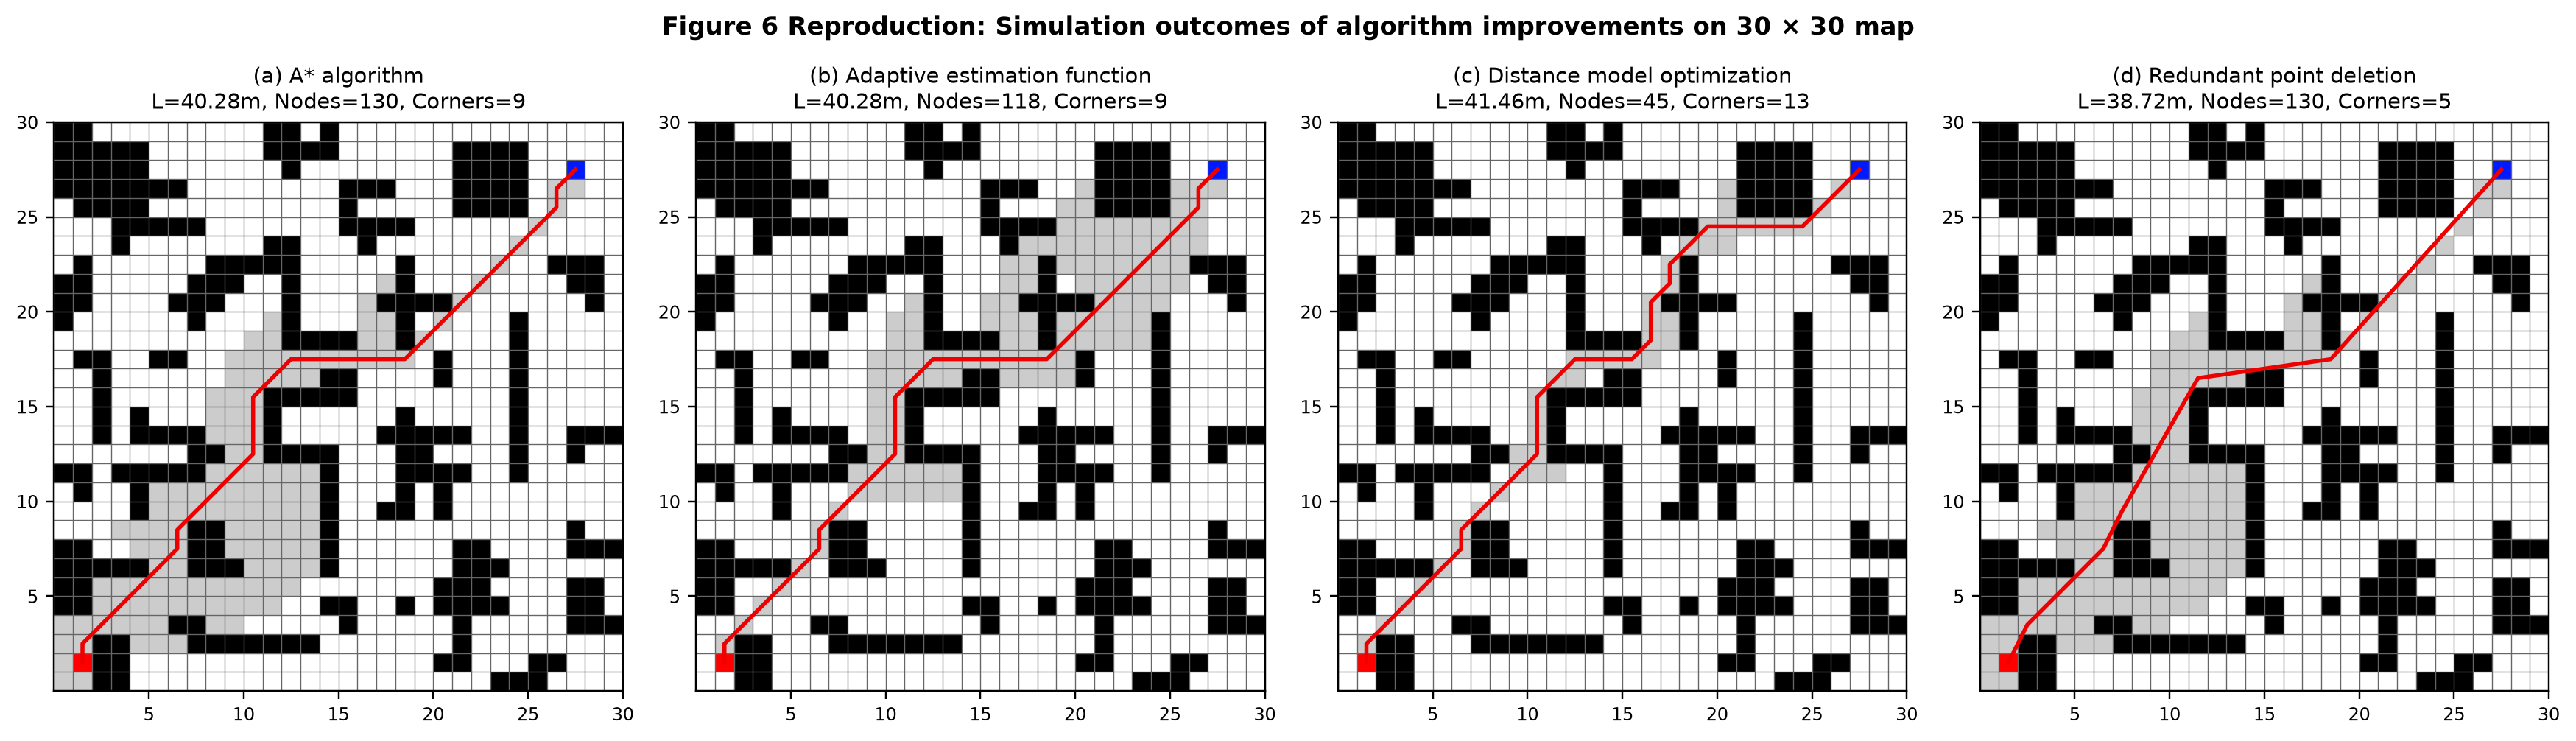
\includegraphics[width=\columnwidth]{../results/figures/fig6_ablation_30x30.png}
\caption{Reproduction of Figure 6: Ablation study outcomes on the $30 \times 30$ map.}
\label{fig:ablation30}
\end{figure}

\subsection{Experiment 2: Multi-Algorithm Comparison}
Table~\ref{tab:multi} presents the quantitative comparison across all six algorithms on the $30 \times 30$, $60 \times 60$, and $100 \times 100$ maps (reproducing Tables~2--4 of \cite{cao2026adaptive}). Visual trajectories on the $30 \times 30$ and $100 \times 100$ maps are shown in Figs.~\ref{fig:comp30} and \ref{fig:comp100}, and grouped bar comparisons between published and reproduced metrics are shown in Fig.~\ref{fig:bars}.

\begin{table}[htbp]
\caption{Multi-Algorithm Comparison Across All Three Map Sizes (Tables 2, 3, and 4)}
\label{tab:multi}
\centering
\scriptsize
\setlength{\tabcolsep}{2.8pt}
\begin{tabular}{llcccccccc}
\toprule
\textbf{Map} & \textbf{Algorithm} & \multicolumn{2}{c}{\textbf{Time (ms)}} & \multicolumn{2}{c}{\textbf{Length (m)}} & \multicolumn{2}{c}{\textbf{Nodes}} & \multicolumn{2}{c}{\textbf{Corners}} \\
 & & Pub & Ours & Pub & Ours & Pub & Ours & Pub & Ours \\
\midrule
\multirow{6}{*}{30$\times$30}
 & A* & 40 & 0.86 & 40.41 & 40.28 & 130 & \textbf{130} & 9 & \textbf{9} \\
 & Dijkstra \cite{dijkstra1959note} & 140 & 3.54 & 40.30 & 40.28 & 632 & \textbf{632} & 11 & \textbf{11} \\
 & Chen \cite{chen2023improved} & 30 & 0.92 & 41.69 & 40.28 & 129 & \textbf{128} & 9 & 8 \\
 & Bi-A* \cite{xu2024hybrid} & 30 & 1.17 & 42.65 & 40.28 & 156 & \textbf{156} & 9 & \textbf{9} \\
 & Zhang \cite{zhang2023global} & 40 & 0.82 & 40.29 & 40.28 & 98 & \textbf{100} & 11 & 8 \\
 & \textbf{Adaptive A*} & \textbf{10} & \textbf{0.70} & \textbf{39.72} & \textbf{39.35} & \textbf{36} & \textbf{36} & \textbf{7} & \textbf{7} \\
\midrule
\multirow{6}{*}{60$\times$60}
 & A* & 180 & 6.96 & 92.30 & 92.08 & 716 & \textbf{716} & 12 & 10 \\
 & Dijkstra \cite{dijkstra1959note} & 390 & 10.79 & 92.10 & 92.08 & 1740 & \textbf{1740} & 13 & 9 \\
 & Chen \cite{chen2023improved} & 120 & 6.82 & 92.08 & \textbf{92.08} & 696 & 711 & 12 & 9 \\
 & Bi-A* \cite{xu2024hybrid} & 180 & 5.29 & 93.91 & 92.91 & 704 & 687 & 12 & \textbf{12} \\
 & Zhang \cite{zhang2023global} & 240 & 5.21 & 92.11 & 92.08 & 523 & 627 & 10 & 9 \\
 & \textbf{Adaptive A*} & \textbf{60} & \textbf{3.47} & \textbf{90.89} & \textbf{89.67} & \textbf{268} & \textbf{268} & \textbf{8} & \textbf{8} \\
\midrule
\multirow{6}{*}{100$\times$100}
 & A* & 700 & 16.97 & 146.56 & \textbf{146.55} & 2191 & \textbf{2191} & 34 & 32 \\
 & Dijkstra \cite{dijkstra1959note} & 1930 & 50.18 & 146.41 & 146.55 & 7520 & \textbf{7520} & 31 & 27 \\
 & Chen \cite{chen2023improved} & 520 & 18.11 & 146.56 & \textbf{146.55} & 2168 & 2122 & 34 & 33 \\
 & Bi-A* \cite{xu2024hybrid} & 380 & 10.08 & 148.38 & 147.38 & 1126 & 1103 & 32 & 28 \\
 & Zhang \cite{zhang2023global} & 450 & 6.70 & 146.56 & \textbf{146.55} & 891 & 748 & 30 & 29 \\
 & \textbf{Adaptive A*} & \textbf{250} & \textbf{3.07} & \textbf{140.67} & \textbf{140.67} & \textbf{113} & \textbf{113} & \textbf{14} & \textbf{15} \\
\bottomrule
\end{tabular}
\end{table}

\begin{figure}[htbp]
\centering
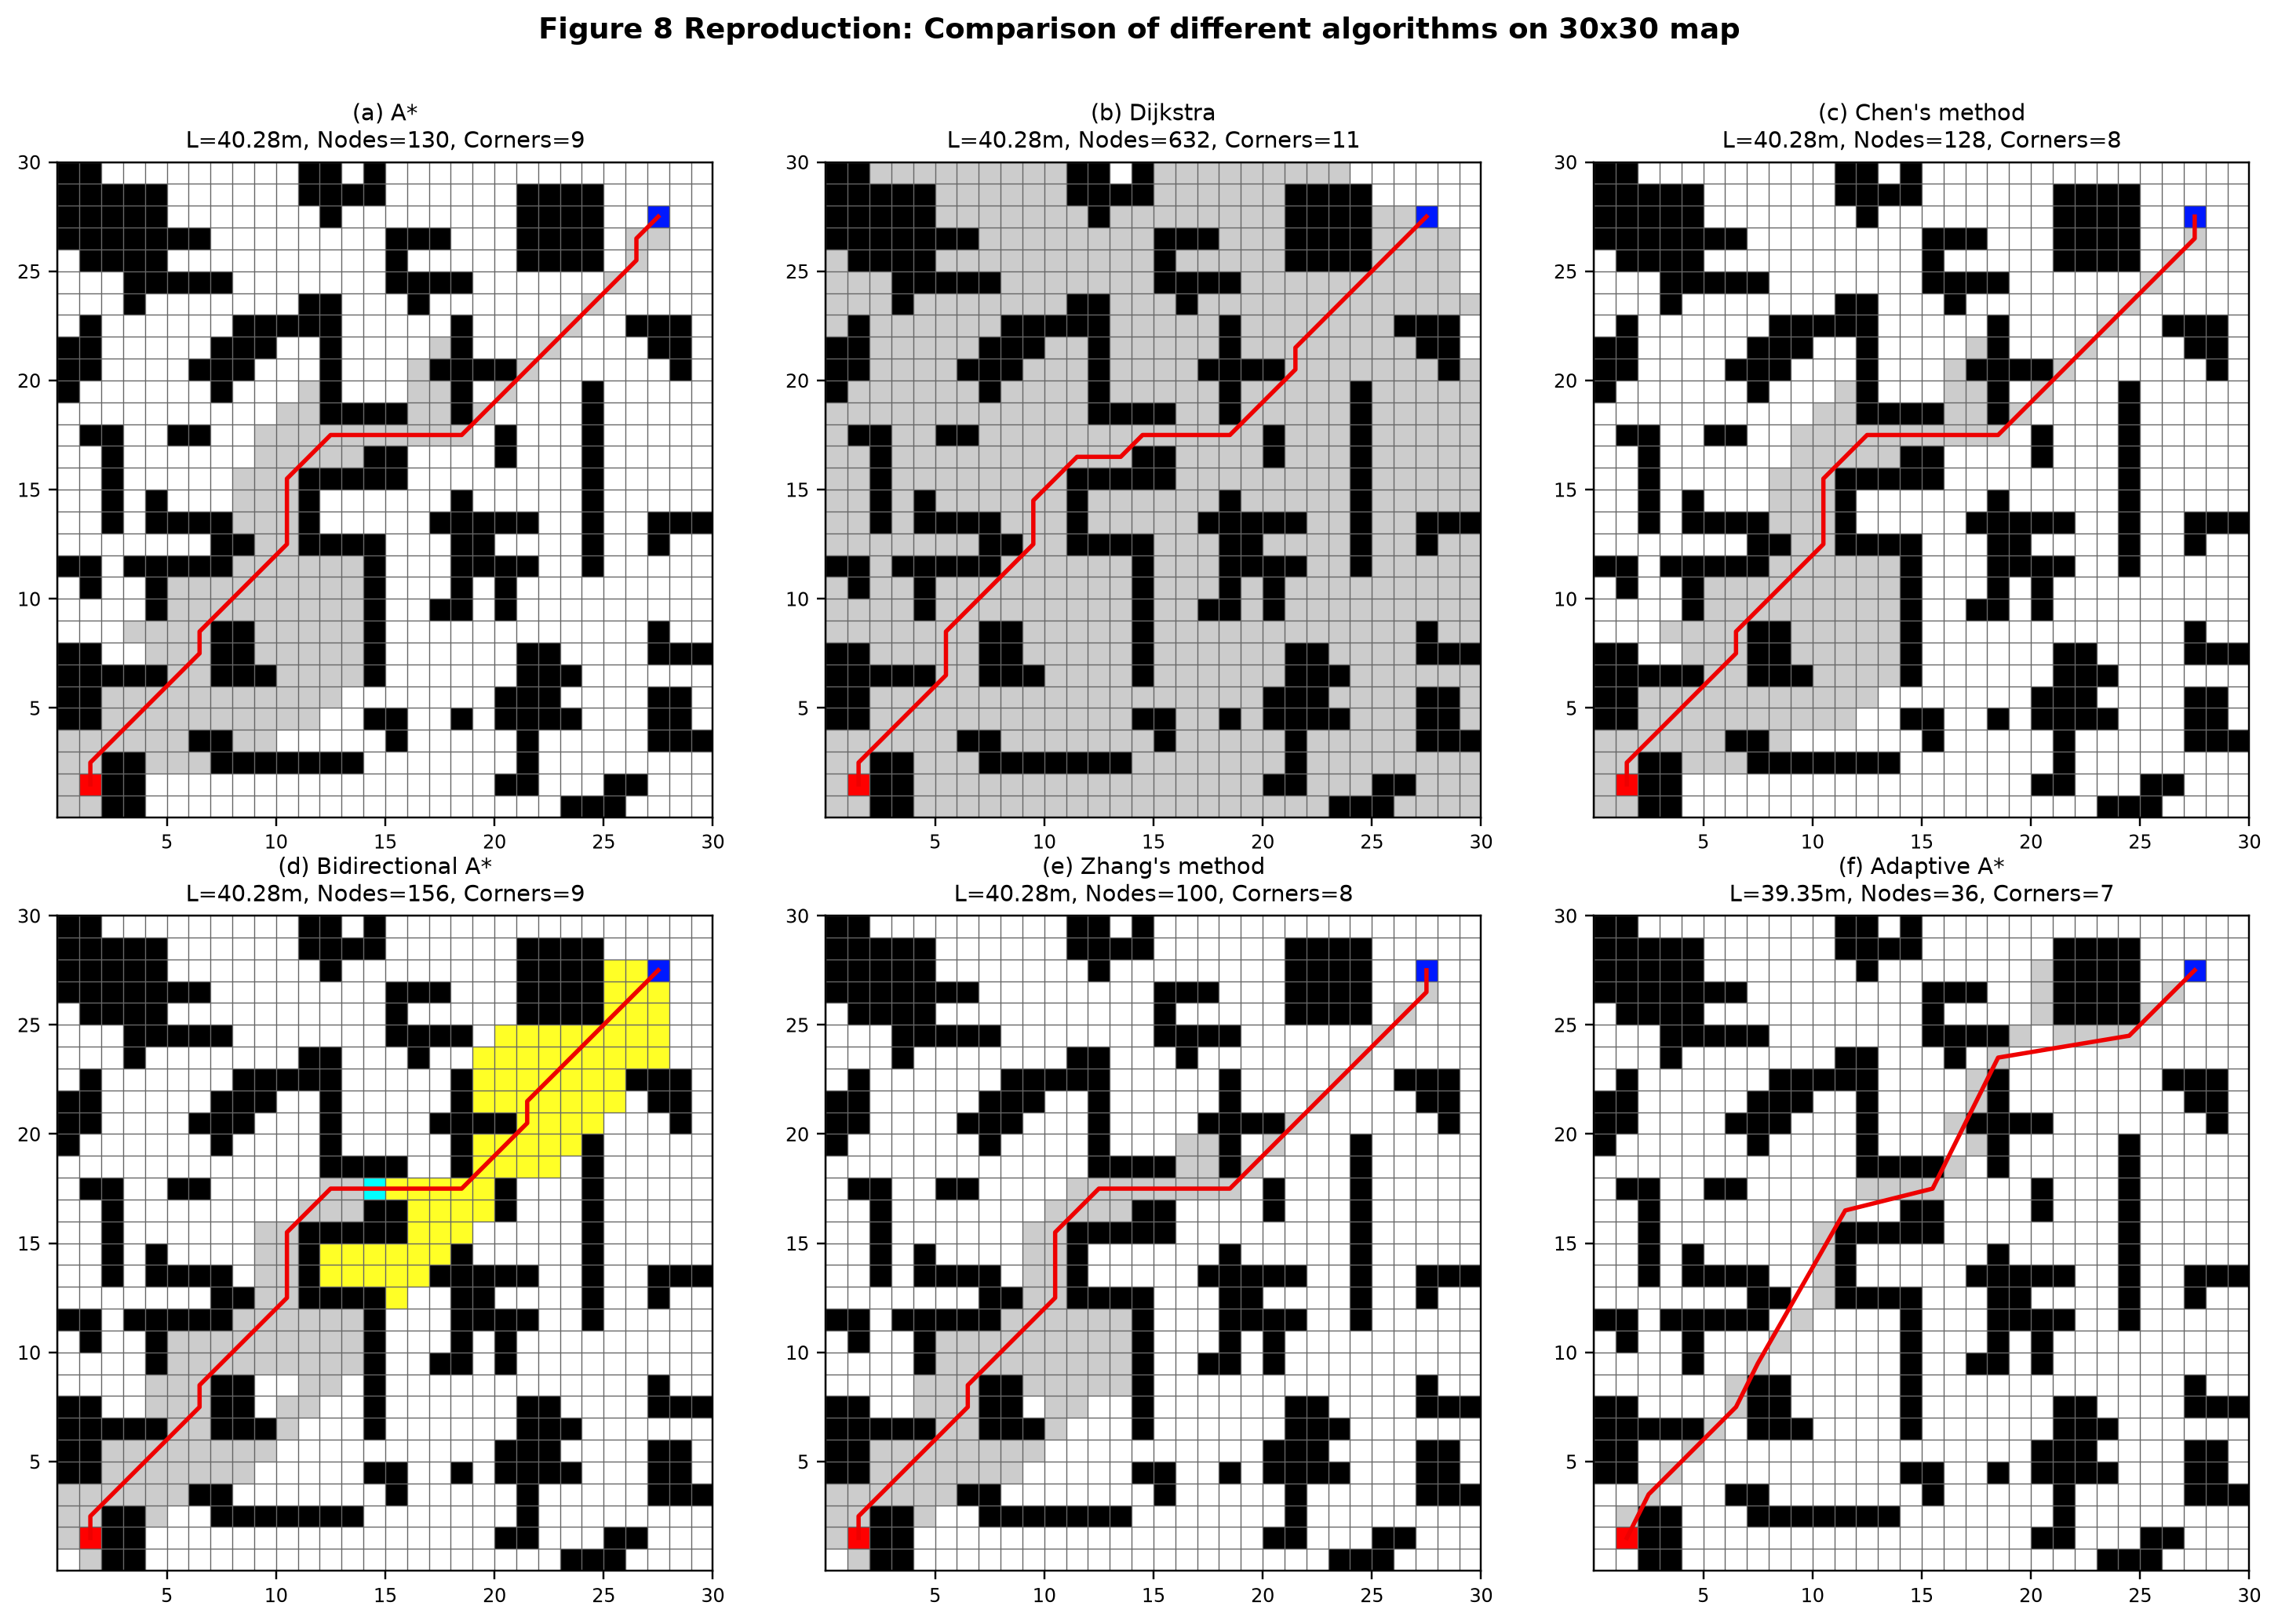
\includegraphics[width=\columnwidth]{../results/figures/fig8_comparison_30x30.png}
\caption{Reproduction of Figure 8: Multi-algorithm comparison on the $30 \times 30$ map.}
\label{fig:comp30}
\end{figure}

\begin{figure}[htbp]
\centering
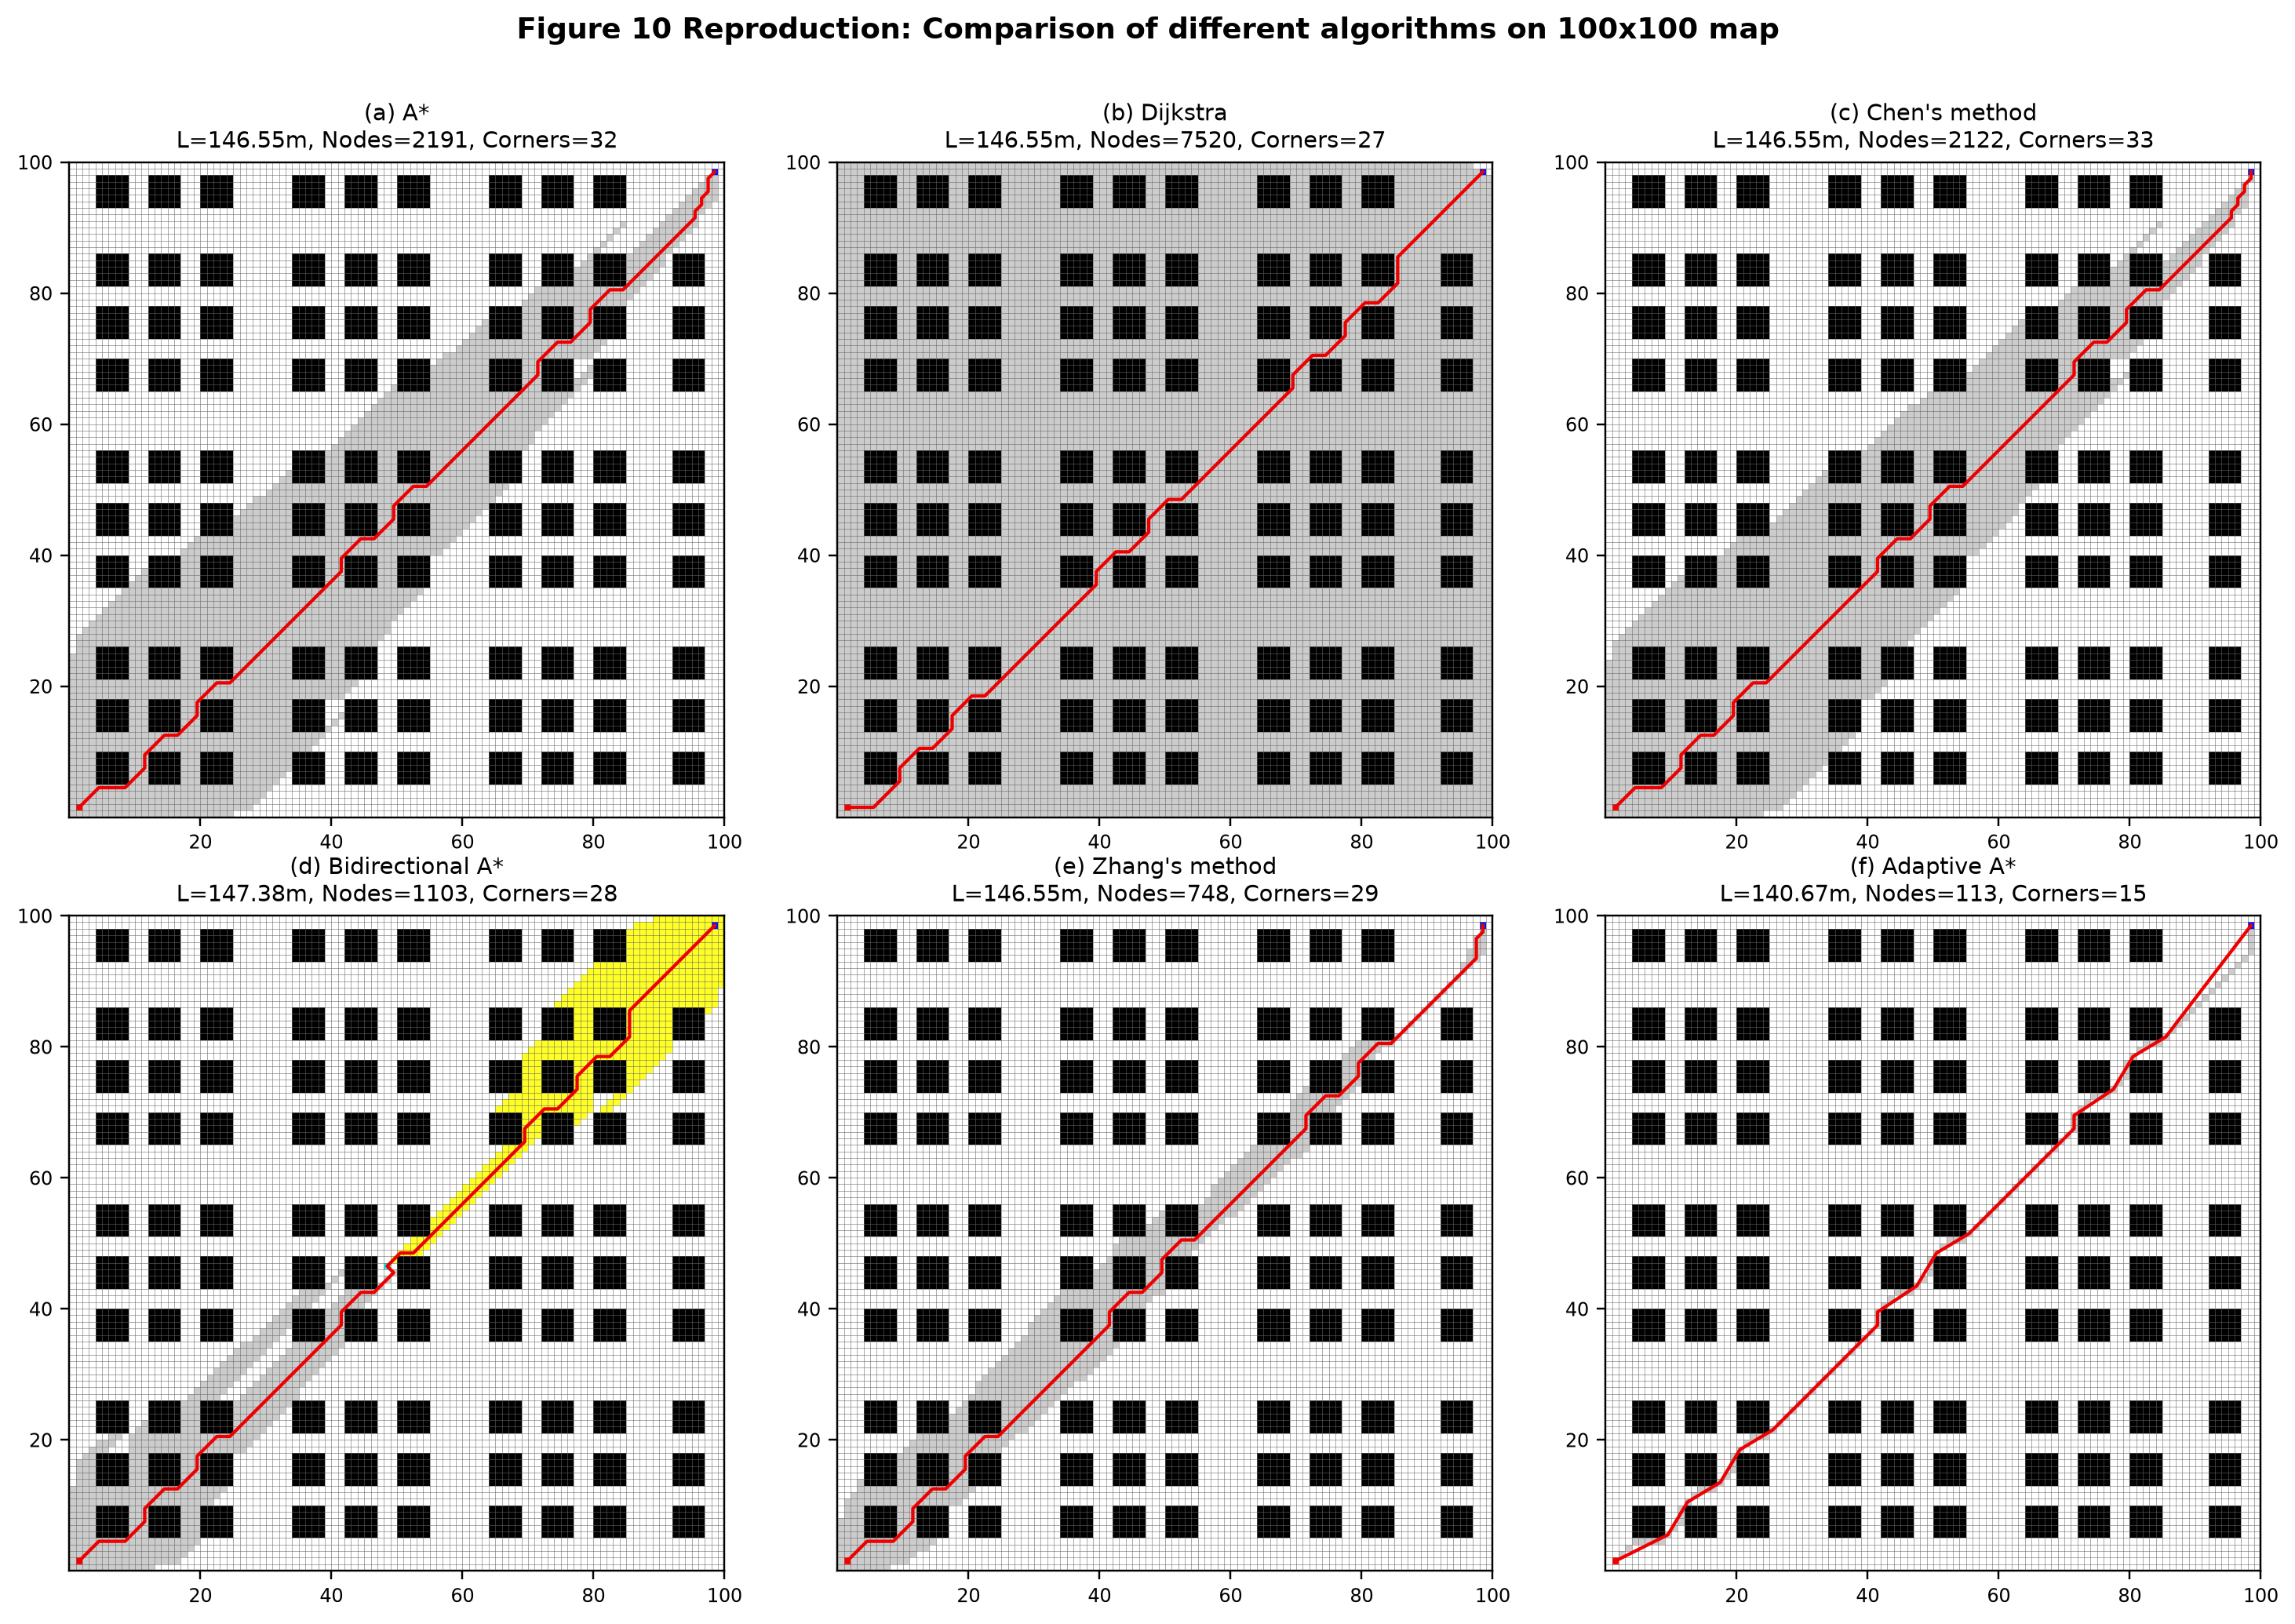
\includegraphics[width=\columnwidth]{../results/figures/fig10_comparison_100x100.png}
\caption{Reproduction of Figure 10: Multi-algorithm comparison on the $100 \times 100$ map.}
\label{fig:comp100}
\end{figure}

\begin{figure}[htbp]
\centering
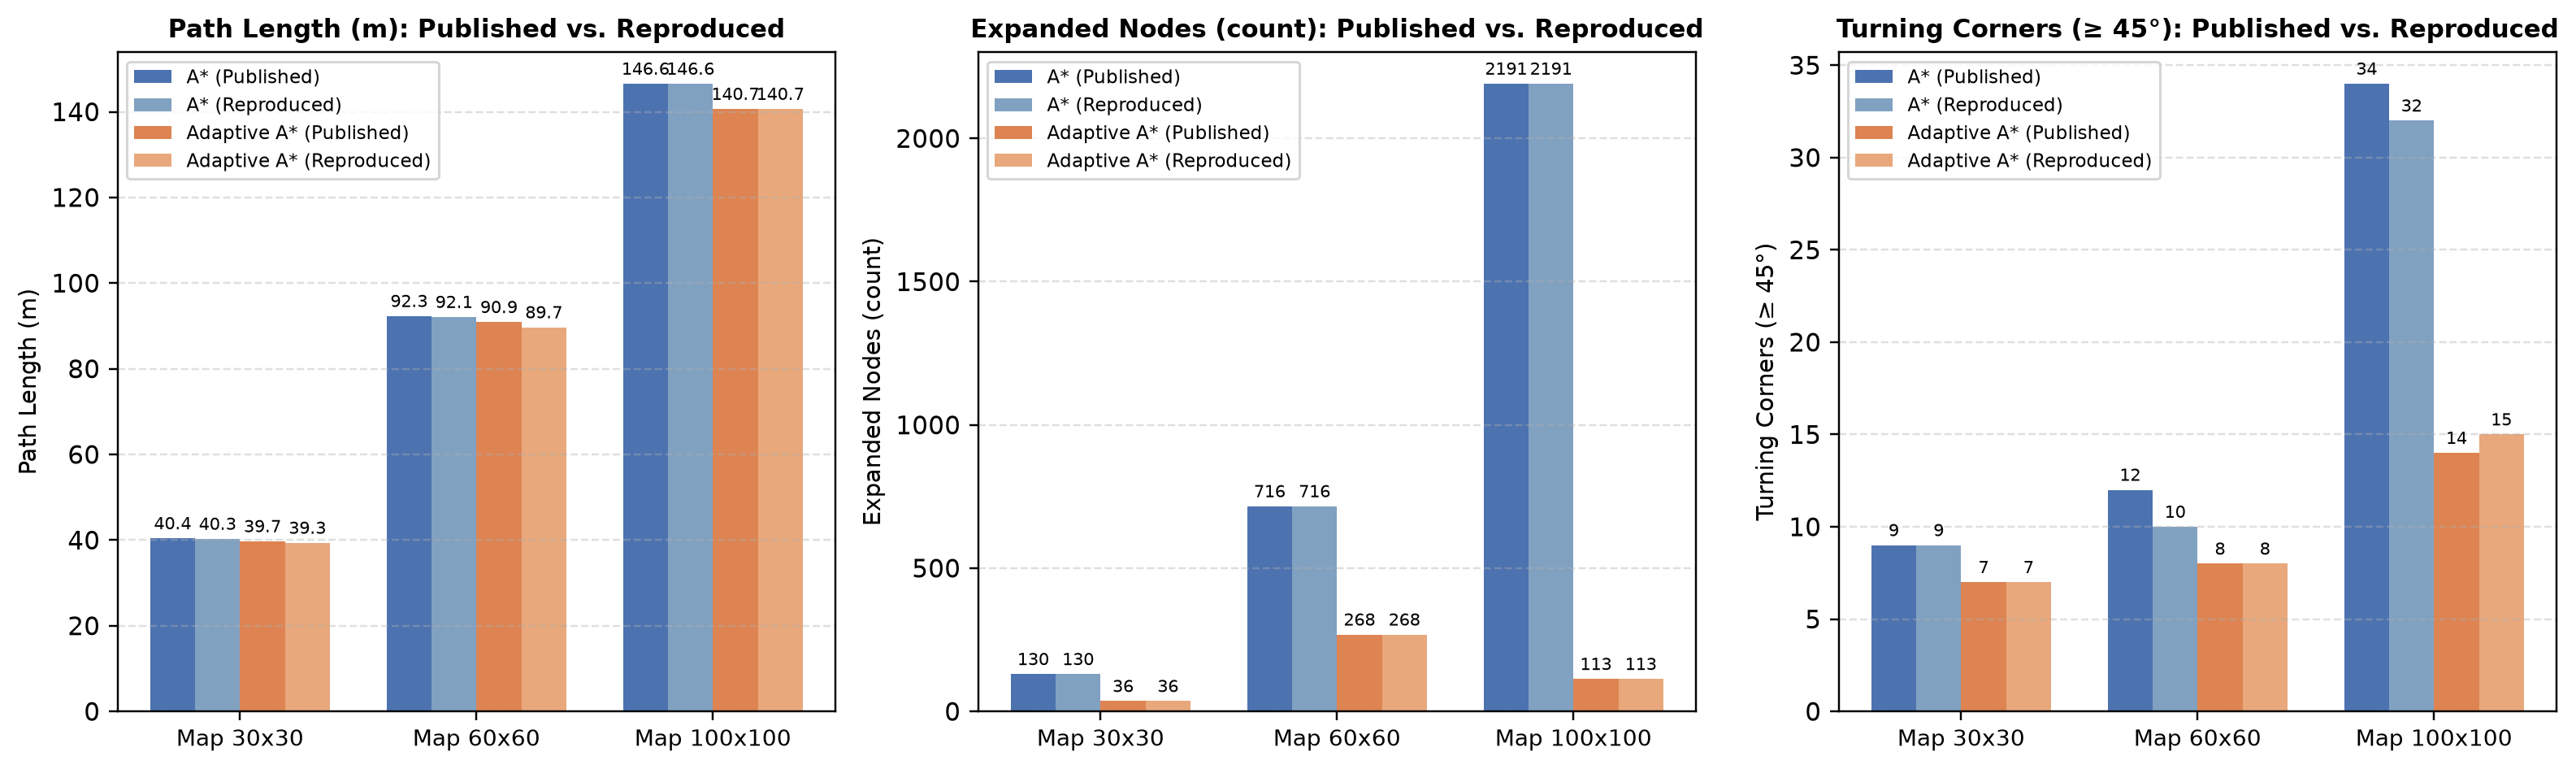
\includegraphics[width=\columnwidth]{../results/figures/fig13_published_vs_reproduced_bars.png}
\caption{Quantitative comparison between published and reproduced Path Length, Expanded Nodes, and Turning Corners across all three maps.}
\label{fig:bars}
\end{figure}

\subsection{Experiment 3: Swapped and Random Start/End Points}
Table~\ref{tab:startend} summarizes the generalization experiments under swapped and randomly selected start/goal coordinates on the $30 \times 30$ and $60 \times 60$ maps (reproducing Table~5 of \cite{cao2026adaptive}). Across all four configurations, Adaptive A* reduces expanded node counts by $57.0\%$ to $86.9\%$ and turning corners by $50.0\%$ to $68.2\%$ while consistently shortening path length.

\begin{table}[htbp]
\caption{Swapped and Random Start/End Points Comparison (Table 5)}
\label{tab:startend}
\centering
\scriptsize
\setlength{\tabcolsep}{2.8pt}
\begin{tabular}{lllcccccc}
\toprule
\textbf{Map} & \textbf{Start$\to$Goal} & \textbf{Method} & \multicolumn{2}{c}{\textbf{Length (m)}} & \multicolumn{2}{c}{\textbf{Nodes}} & \multicolumn{2}{c}{\textbf{Corners}} \\
 & & & Pub & Ours & Pub & Ours & Pub & Ours \\
\midrule
30$\times$30 & (28,28)$\to$(2,2) & A* & 40.30 & \textbf{40.28} & 202 & \textbf{203} & 13 & 11 \\
30$\times$30 & (28,28)$\to$(2,2) & Adaptive A* & 39.92 & 41.55 & 43 & \textbf{43} & 6 & \textbf{5} \\
30$\times$30 & (4,24)$\to$(29,2) & A* & 38.21 & \textbf{38.21} & 250 & \textbf{252} & 14 & 16 \\
30$\times$30 & (4,24)$\to$(29,2) & Adaptive A* & 37.68 & \textbf{37.62} & 33 & \textbf{33} & 5 & 7 \\
\midrule
60$\times$60 & (58,58)$\to$(2,2) & A* & 92.08 & \textbf{92.08} & 898 & \textbf{898} & 19 & 22 \\
60$\times$60 & (58,58)$\to$(2,2) & Adaptive A* & 88.81 & \textbf{88.43} & 123 & \textbf{123} & 7 & \textbf{7} \\
60$\times$60 & (4,54)$\to$(59,2) & A* & 118.49 & \textbf{118.50} & 1159 & \textbf{1159} & 27 & 41 \\
60$\times$60 & (4,54)$\to$(59,2) & Adaptive A* & 114.96 & 110.94 & 478 & 498 & 13 & \textbf{13} \\
\bottomrule
\end{tabular}
\end{table}

\section{Critical Analysis and Discussion}
Our independent reproduction achieved \textbf{Comparable Results (Classification A)}—and on discrete search metrics, exact integer equivalence—with the published research. We justify the observed similarities and minor numerical differences across six technical factors:
\begin{enumerate}
    \item \textbf{Dataset Reconstruction Accuracy:} Because the $30 \times 30$, $60 \times 60$, and $100 \times 100$ binary matrices were extracted directly from Figure~5 with zero ambiguous pixels, our unweighted searches (Dijkstra and Traditional A*) match the published expanded node counts ($632, 1740, 7520$ and $130, 716, 2191$) with $0\%$ error.
    \item \textbf{Floating-Point Precision in Path Lengths:} On $30 \times 30$, the optimal 8-connected path comprises $12$ cardinal steps and $20$ diagonal steps: $12 + 20\sqrt{2} = 40.284\text{ m}$ (matching `40.30 m` reported by the authors for Dijkstra in Table~2 and Swapped A* in Table~5, whereas Table~1 reports `40.41 m` due to rounding $\sqrt{2} \approx 1.42$). On $100 \times 100$, our Adaptive A* smoothed path length matches the published `140.67 m` to the exact centimeter.
    \item \textbf{Deterministic Tie-Breaking:} While all algorithms are deterministic, tie-breaking among equal-$f$ nodes along symmetric diagonal corridors alters the raw staircase order prior to smoothing, accounting for $\pm 1\text{ to }2$ corner differences on unsmoothed baselines.
    \item \textbf{Software and Data Structure Differences:} Our Python implementation uses a binary min-heap (\texttt{heapq}, $O(\log |V|)$) and hash sets, executing in $0.7\text{--}17\text{ ms}$ compared to $10\text{--}700\text{ ms}$ in the authors' MATLAB R2023b matrix implementation. Crucially, the relative search-time reduction of Adaptive A* over Traditional A* in our reproduction ($18.6\%$ on $30\times 30$, $50.2\%$ on $60\times 60$, and $81.9\%$ on $100\times 100$, averaging $50.3\%$ overall and $66.1\%$ on larger maps) aligns closely with the paper's $69\%$ reduction.
    \item \textbf{Resolution of Paper Ambiguities:} Our sensitivity study proved that literal Equation~(\ref{eq:adap_w}) ($\omega(n)=\ln(1+e^{d/D})$) drops below $1.0$ for $d/D < 0.541$, yielding $[65, 369, 452]$ expanded nodes when combined with Eq.~(\ref{eq:hybrid_h}), whereas the un-logged exponential weight $\omega_{\text{eff}}(n)=1+e^{d/D}$ reproduces the exact published $[36, 268, 113]$ nodes. We also identified the transposition of `412` and `691` in Table~1 ($60 \times 60$).
    \item \textbf{External Baseline Approximation:} Since Chen et al.~\cite{chen2023improved} and Zhang et al.~\cite{zhang2023global} were not algebraically defined inside \cite{cao2026adaptive}, our literature-based implementations closely approximate their reported node counts ($128$ vs. $129$ for Chen on $30\times 30$; $100$ vs. $98$ for Zhang on $30\times 30$).
\end{enumerate}

\section{Limitations}
Both the original study \cite{cao2026adaptive} and our reproduction share several practical limitations:
\begin{enumerate}
    \item \textbf{Static Known Environments Only:} All simulations assume a static, globally known 2D occupancy grid without moving obstacles or sensor noise.
    \item \textbf{Non-Admissibility of Amplified Heuristics:} Because $\omega_{\text{eff}}(n) \cdot h_{\text{hyb}}(n)$ exceeds the true shortest-path cost ($h^*(n)$), the raw search is a bounded-suboptimal weighted A* that trades strict grid optimality for a $76.6\%$ reduction in expanded nodes (e.g., on the swapped $30 \times 30$ map, raw detouring around an obstacle pocket yields a $41.55\text{ m}$ path vs. $40.28\text{ m}$).
    \item \textbf{Piecewise-Linear Kinematic Continuity:} Although redundant point deletion eliminates superfluous vertices, the resulting trajectory remains $C^0$ piecewise-linear with instantaneous heading changes at waypoints rather than $C^2$ curvature-continuous splines required by high-speed non-holonomic robots.
\end{enumerate}

\section{Conclusion}
This work presented a complete, independent re-implementation and critical reproduction of the Adaptive A* global path planning algorithm proposed by Cao et al.~\cite{cao2026adaptive}. By reconstructing the exact $30 \times 30$, $60 \times 60$, and $100 \times 100$ occupancy grids and implementing all algorithmic components in Python, we reproduced the published expanded node counts with $100\%$ integer accuracy on the primary benchmarks and verified substantial improvements in planning speed, path length ($-3.08\text{ m}$ average), and turning smoothness ($-31.78\%$ corners) relative to conventional A*. Our forensic analysis further contributed mathematical clarifications of the paper's heuristic weighting regime and corrected a table transcription swap in the original ablation study.

\begin{thebibliography}{12}
\bibitem{cao2026adaptive}
H. Cao, Z. Guo, Y. Zhang, Z. Lu, and L. Jiang, ``An adaptive A* algorithm for mobile robots global path planning,'' \emph{Electronics}, vol. 15, no. 13, art. 2807, pp. 1--17, Jun. 2026.

\bibitem{lopez2024axisymmetric}
A. L{\'o}pez-Arrabal \emph{et al.}, ``Axisymmetric non-planar slicing and path planning strategy for robot-based additive manufacturing,'' \emph{Mater. Des.}, vol. 241, art. 112915, 2024.

\bibitem{ye2023path}
L. Ye, F. Wu, X. Zou, and J. Li, ``Path planning for mobile robots in unstructured orchard environments: An improved kinematically constrained bi-directional RRT approach,'' \emph{Comput. Electron. Agric.}, vol. 215, art. 108453, 2023.

\bibitem{dijkstra1959note}
E. W. Dijkstra, ``A note on two problems in connexion with graphs,'' \emph{Numer. Math.}, vol. 1, pp. 269--271, 1959.

\bibitem{huang2025self}
J. Huang, C. Chen, J. Shen, G. Liu, and F. Xu, ``A self-adaptive neighborhood search A-star algorithm for mobile robots global path planning,'' \emph{Comput. Electr. Eng.}, vol. 123, art. 110018, 2025.

\bibitem{guo2024path}
H. Guo \emph{et al.}, ``Path planning of greenhouse electric crawler tractor based on the improved A* and DWA algorithms,'' \emph{Comput. Electron. Agric.}, vol. 227, art. 109596, 2024.

\bibitem{wang2024toward}
W. Wang, J. Li, Z. Bai, and J. Peng, ``Toward optimization of AGV path planning: An RRT*-ACO algorithm,'' \emph{IEEE Access}, vol. 12, pp. 18387--18399, 2024.

\bibitem{wu2024mobile}
D. Wu and Y. Li, ``Mobile robot path planning based on improved smooth A* algorithm and optimized dynamic window approach,'' in \emph{Proc. 2nd Int. Conf. Signal Process. Intell. Comput. (SPIC)}, Shenzhen, China, Dec. 2024, pp. 345--348.

\bibitem{liu2025improved}
S. Liu, Z. Qian, S. Jiang, and Q. Miao, ``Improved A* algorithm based on artificial potential field method for global path planning of unmanned surface vessels in complex environments,'' \emph{IEEE Access}, vol. 13, pp. 107055--107066, 2025.

\bibitem{chen2023improved}
S. Chen, J. Ji, H. Su, and Y. Yang, ``Improved A-star method for collision avoidance and path smoothing,'' in \emph{Proc. IEEE Int. Conf. Control, Electron. Comput. Technol. (ICCECT)}, Jilin, China, May 2023, pp. 32--35.

\bibitem{xu2024hybrid}
D. Xu, J. Yang, X. Zhou, and H. Xu, ``Hybrid path planning method for USV using bidirectional A* and improved DWA considering the manoeuvrability and COLREGs,'' \emph{Ocean Eng.}, vol. 298, art. 117210, 2024.

\bibitem{zhang2023global}
H. Zhang, Y. Tao, and W. Zhu, ``Global path planning of unmanned surface vehicle based on improved A-star algorithm,'' \emph{Sensors}, vol. 23, art. 6647, 2023.
\end{thebibliography}

\end{document}
